\section{Grundlagen}
\label{sec:Grundlagen}


\subsection{Optimierungsgrundlagen}
Angenommen es soll ein Neuronales Netz mit k Layern und jNeuronen zur Klassifizierung von einfachen Handgeschrien-Zahlen erstellt werden. Der Entwickler entscheidet sich für ein 3 Layern Netz mit jeweils 3 Neuronen. Nach dem Training hat es die Genauigkeit von 85 Prozent. Ist dies Akzeptabel? Kann man sagen das für k 3 bzw. j 3 die optimale Lösung ist? Um dies zu beurteilen müssen viele Experimente durchgeführt werden. Die Frage ist, wie man den die Besten werte für k und j findet, der die Klassifizierung maximiert. Dies wird als Hyperparameter Optimierung bezeichnet. Bei der Optimisierung wird mit einem Inizialwert gestartet dieser ist meist nicht der beste. Dieser Inizialwert muss einige male geändert werden um auf einen Optimum zu kommen. Manchmal ist dieses Anpassen/optimieren so Komplex, dass es durch eine Funktion ersetz werden muss.

\subsection{Genetische Algorithmen}
Genetische Algorithmen sind heuristische Suchansätze. Im wesentliche zeichnet sie eine probilistische Eltern selection als primären Suchoperator aus. Als weitern suchoperator kann der Ga noch auf die Mutation zurückgreifen, dieser grantiert eine Erreichbarkeit aller Punkte im suchraum und erhält so die Grunddiversität in der Population. Genetische Algorithmen haben als theoretischen Grundlage die Schama-Therorie. Es gibt zwei verschiedene Grundalgorihmen der Standart-GA (\ref{Standart-GA}). Dieser Tauscht nach einer Generation die komplette Elternpopulation durch die Kinderpopulation aus. Im Gegensatz dazu gibt es  den Steady-State-GA(\ref{Steady-State-GA}) welcher durch seine Überlappende Population auszeichnet. Nun werden wir uns genauer den  Standart-GA \ref{Standart-GA} und seine einzelnen Schritte genauer Betrachten.

\subsection{Standart-GA} \label{Standart-GA}
Der Standart-GA ist folgende Schritte aufgeteilt und wird anschließend genau besprochen:
Schritt 1 Inizialisieren einer Population.
Schritt 2 Fittness brechnen.
Schritt 3 weiterentwicken hier werden zuerst die passenden Eltern ausgesucht und anschließend mit Crossover und Mutation die Kinder Population erstellt. 
Schritt 4 Elternpopulation durch die neue Kinderpopulation ausgetauscht.
Hier noch einamal als Pseudocode.

Algorithm 1 Basic Genetic Algorithm
1: initialize population
2: repeat
3: 		repeat
4:			fitness computation
5:			parent selection
6:			breed
7:				crossover
8:				mutation
9:		until population complete
10:		selection of parental population
11: until termination condition



\iffalse
Genetische Algorithmen sind im Wesentlichen durch eine probabilistische Eltern selektion und die Rekombination als primären Suchoperator gekennzeichnet.Die Mutation ist meist nur ein Hintergrundoperator, der mit einer geringen Wahrschenlichkeit zur anwendungkommt. Er garantiert die Erreichbarkeit aller Punkte im Suchraum und erhält eine Drunddiversitöt in der Population.

Evolutionäre Algo -- s.128


Genetische Algorithmen sind heuristische Suchansätzem, die auf einer breitenbasis von Optimierungsproblemen angewendet werden können. Diese Flexibiliät macht sie für die Praxis für viele sehr attraktiv.Die Evulution ist Grundlage des Genetischen Aglorithmuses. durch die aktuelle Vielfalt und der Erfolg der Arten ist dies schon alleine ein guter Grund sich diesen Optimierungs Algortihmus näher anzuschauen. Denn sdiese Arten sind in der lage sich an ihre Umgebung anzupassen und sich zu zu komplexen Strukturen zuentwickelen, und somit das überleben in verschiedesten Umgebungen eröglichen. Hierbei ist die Paarung und Entwicklung von Nachkommen eine der Hauptprinipen des Erfolges der Evolution. In diesem Kapitel werden wir die Grundlage der GEnetischen Algorithmen näher anzuschauen. Beginnen wir mit der grundlage das es sich bei den Genetischen Algorithmen um einen Polulations ansatz handelt. Anschließend wird auf die wichtigesten genetischen Operatioren vorstellen darunter gehöhren, Selektion, Crossover und Muttation

Seite - 11 Genetic Algorithm Essentials


Algorithmus 1 zeigt den Pseudocode des grundlegenden genetischen Algorithmus, der Folgendes kann dienen als Blaupause für viele verwandte Ansätze. Am Anfang eine Reihe von Lösungen,die als Population bezeichnet wird, wird initialisiert. Diese Initialisierung wird empfohlen.um zufällig den gesamten Lösungsraum abzudecken oder um Experten zu modellieren und einzubinden. Wissen. Die Darstellung bestimmt den Initialisierungsprozess. Für BitfolgeDarstellungen ist eine zufällige Kombination von Nullen und Einsen sinnvoll, z.B.das anfängliche Zufallschromosom 1001001001001 als typische Bitfolge der Länge 10. Der Hauptgenerationskreislauf des Genetischen Algorithmus erzeugt neue Nachkommen.Kandidatenlösungen mit Crossover und Mutation, bis die Bevölkerung vollständig ist.

Algorithm 1 Basic Genetic Algorithm
1: initialize population
2: repeat
3: 		repeat
4:			fitness computation
5:			crossover
6:			mutation
7:			phenotype mapping
8:		until population complete
9:		selection of parental population
10: until termination condition

Seite - 11 Genetic Algorithm Essentials
\fi 

\subsubsection{Initzialisierung der Population}
Der Klassiche Genetische Algorithmus bassiert auf einer Reihe von Kandidatenlösungen. Dee größe der Populaton ist auch die Anzahl der Lösungen. Jede Lösung kann als einzelnes Induvidum gesehen werden und wird durch ein Chromsone representiert. Es gibt verschiedene möglichkeiten diese Gene dazustellen, wie z.B binär oder Dezimal.
Figure \ref{fig:chromosome} veranschaulicht ein Beispiel, wie eine Population aus vier Individuen(chromosomes)mit je einem Chromosom. Ein Chromso, besitzt wiederum  vier gene. Jedes dieser Gene ist durch eine binären zahl repräsentiert. 

\noindent%
\begin{figure}[H]
  \centering  
  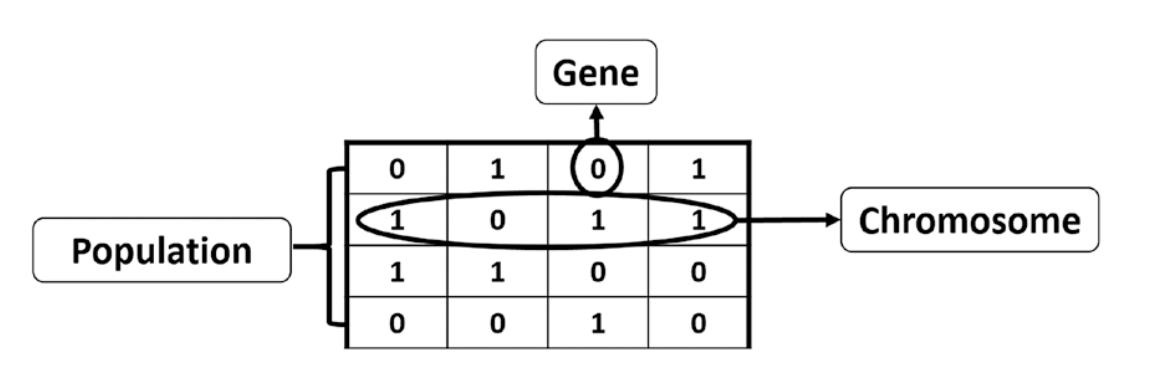
\includegraphics[scale=0.3]{img/Chromsome-s134-PracticalComputerVion.png}
  \caption{Beispiel einer Polulation mit 4 induviduen (Chromsomen) welche vier binäre Gene besitzen \cite{Rashid2017} }
  \label{fig:chromosome}
\end{figure}

Diese anfangs Poulation wird meißt Zufällig inizialisiert. Hier durch ist es möglich die größte abdeckung des Suchsraums zu gewähren. Dadurch besitzt die erste Generation eine sehr geringe Fittness dies verbessert sich aber im Lauf des Trainings. Durch Selection werde die nicht unnötigen/Contra-produktiven Individumen aussotiert. Bevor dies passiert muss aber erst die Bewertung durchgeführt werden.


\subsubsection{Bewertung aka Grade / Fittnesfunktion}
Nun besteht die erste Generation(Generation 0) aus einer Population mit völlig zufälligen Induviduen. Diese werden anhand einer für sine anwendung speizellen Fitnessfunktion bewerte. Dabei werden nicht einzelnen Gene bewertet sondern das ganze Genom/Chromoson/Idividum. Es wird also nicht berücksichtigt welches Gene sich positiv bzw. negativ auswirklen. Als Rückgabewert gibt die Fittnesfunktion uns einen Fittneswert, dabei steht ein höherer Fittnesswert stehts für eine höher Qualität an Individum. Da nun alle Individuen der Population bewertet wurden kann eine neue Generation erstellt werden.


\subsubsection{Weiterentwickeln aka Evolve}
Dazu werden aus zwei Elternpaaren ein neues Kind erstellt. Um die Elternpaare auszusuchen gibt es verschiedene Optionen.Da nun die Eltern fest stehen, wird per Crossover aus den beiden Elternpaaren oder aus dem Elternpool ein neues Kind generiert. Um bei den Genen eine höhere diversität zu gelangen werden die Kindergene noch mit einer Mutation versehen. Somit kann man einen höheren Suchraum(Abdeckungsgrad) abdecken. Nach dem eine neue Kind generation erstellt wurde wird der ganze vorgang so lange wiederhollt bis die geforderte Fintess ereicht wurde.

\paragraph{Auswahl der Elternpaare aka Select Parents}
Um eine convergenz richtung Optimalem Maximum bzw. Minmum zu schaffen werden die besten Elternteile der geraden bewertenen Generation ausgewählt.
Für die Auswahl gibt es verschiedene Ansätze, die bedeutesten werden genannt und erläutert.
\begin{itemize}
\item \textbf{Auswahl proportional zu Fittnes eng. Fitness Proportonal Selction(FPS)}, hierbei spielt die im vohrigen Schritt berechnete Fintess eine große Rolle. Die Eltern werden nach dieser Fittness proportional als Elternteil ausgewählt und zum Elternpool hinzugefügt.

\iffalse
Problem hier ist das Individuen die am anfang gut sind schnell die ganz epopulation übernehmmen. Das kann dazuführen das eine mögliche bessere lösung durch den Algorithmus im suchraum nicht gefudnen wird. Ein weiteres Problem ist es wenn die Lösungen nahe bei bei einandern liegen gibt es fast keine selections druck mehr herscht. DIes geschied gegen ende der Optimierung und führt zu einem sehr langsamen verlauf gegen ende. 

introduction to evolutionary comp s80
\fi




\item \textbf{Ranking Selektion}, diese Selktion wurde als Verbesserung der Fitness Proportonal Selection entwickelt. Dabei werden die Eltern nicht direkt nach ihrer Fittness ausgewählt sondern über die Fitness im vergleich zur gesamt Population. Sprich sie werden in einer Rangliste aufgestellt wobei das beste Individum den Rand y-1 belegt und das schlechteste den Rang 0. Dieses Ranking kann in vielen varianten vorgenommen werden, Linear oder expotenziel umgesetzt werden. 

\iffalse 

intodiction to evolutionary comp s82




\item \textbf{Best 50 prozent},heißt aus der oberen hälfte der alten Generation werden alle Induviduen dem Elternpool hinzugefügt.Aus welchen dann zufällig die einzelnen Elternteile ausgewählt werden. Es mssen natürlich nicht immer 50 prozent sein, es kann sich auch um einen anderen Prozentsatz handeln.

fliegt ganz raus so wird es momentan im code umgesetzt 16.juli -> verschieben in kapitel konzept

\fi

\item \textbf{Tunier selektion}, in diesem Verfahren werden k induviduen der Population ausgewählt. Diese k Induviuen treten dann wie in einem Tunier gegeneinander an. Das Individum mit dem Besten Fittneswert ein Elternteil ausgewählt. Hierbei wird auf den Elternpool verzichtet und direkt ein Kind aus zwei gewinnern erstellt. Eingesetzt wird dies bei eher kleinen Populationen.
\item \textbf{Comma selction}, Genetic algorithm essentails s.17
\item \textbf{Pluss selection}, Genetic algorithm essentails s.17
\end{itemize}


Nun wurden die Eltern ausgewählt aus der Elterngeneration kann jetzt eine neue Kindergeneration erstelt werden. 

\paragraph{Paarung aka Breed / Variation}
Aus dem Elternpool/paarungspool werden nun Nachkommen(Kinder) geschaffen. Alleine durch die Paarung(Crossover) von qualitativ hochwertigen Individuen wird erwartet, dass die Nachkommen eine bessere Qualität besitzen als die ihrer Eltern. Dennoch kann es zu negative man nur die Eigenschaften der Eltern übernimmt kann es sogar dazu kommen das negative eigenschaften mit übernommen werden. Da dies natürlich nicht gewollt ist gibt es eine einfach Verbesserungs möglichkeit. Die Muation, hier wird jedes Gen noch einmal mit einer zufälligen Muation versehen welches ähnliche aber andere Lösungen hervorbringt. Nun gehen wir noch einmal genauer auf Operation Chrossover und Muation ein.


\iffalse
Somit müsste sich die Finttnes der nächsten generation verbessern. Um dies zu ereichen werden die  Gene noch modifiziert, durch corssover oder mutation. Somit wird der suchraum noch einmal vergrößert aber nur in der nähe der für gut empfunden Individuem bzw. dieser Gene.
Um aus den Einzelnen elternpaaren neue Individuen zu generieren wird das Verfahren/algorithmus Crossover verwendet. Bei Crossover kann es nun auch verschiedene möglichkeiten geben.
\fi


\begin{itemize}
\item \textbf{Crossover}, werden die Chromostränge der Kinder Individuen bestimmt. Beim Crossover gibt es mehrer varianten eine ist die Two-Point-Crossover bei der 50 Prozent des ersten Elternteils und 50 Prozent des zweiten elternteils verwendet, wie es im Oberenteil der Abbildung \ref{fig:chromoson_crossover} zu sehen ist. Ein zweiter Ansatz ist die Uniform-Crossover, hier werden die Gene ganz zufällig und unabhänig von einander ausgewählt, wie im Unterenteil der Abbildung dies nennt man  \ref{fig:chromoson_crossover} zu sehen ist. 

\begin{figure}[H]
  \centering  
  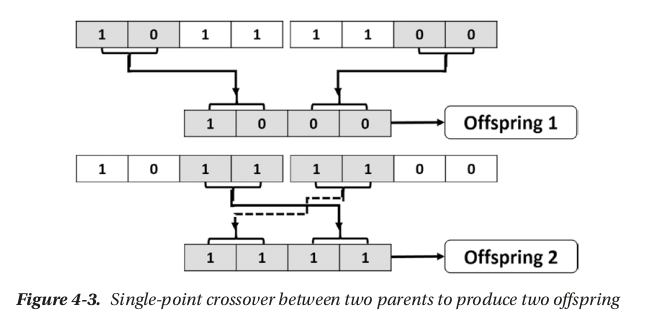
\includegraphics[scale=0.5]{img/crossover.png}
  \caption{crossover anhand eines einfachen binären Chroms. Das erste zeigt eine 50/50 crossover. Das zweite zeigt eine Zufällige auswahl ders Gens.\cite{Rashid2017} }
  \label{fig:chromoson_crossover}
\end{figure}

\item \textbf{Mutation},hierbei wird jedes gens des Indivium zufällig mit einer zufälligen Mutation versehen. Durch diese Mutation wird eine neue Inforamtion/Lösung in die nachfolgende Generation übergeben. Durch diese Mutation ist es möglich einen größeren Suchraum abzudenken. Es ist auch möglich die Werte genauer anzupassen um so auf die Optimalste Lösung zu kommen. 

\end{itemize}

\begin{figure}[H]
  \centering  
  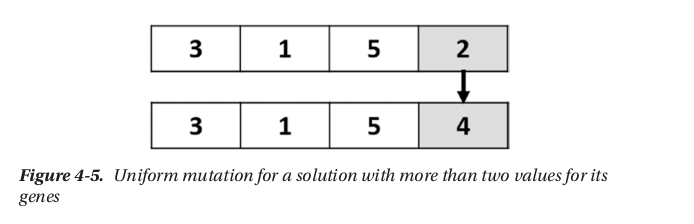
\includegraphics[scale=0.5]{img/mutation.png}
  \caption{Muation eines Genes um höhere vielfältigkeit zubekommen.\cite{Rashid2017} }
  \label{fig:chromoson_mutation}
\end{figure}


\subsubsection{Austausch/ Scheife / Exchange}
Die neue Generation aus Kindern tauscht nun die alte Generation aus. Nun folgen die gleichen Schritte: Grade, Slection, crossover und mutation. 
Diese Schleife wird so lange durchegführt bis die Populationsfittnes das zuvor festgelegte Maximum erreicht. Wenn dies geschied gibt es viele Lösungen welche alle sehr ähnlich sein sollten. Aus dieser kann dann das beste Individum ausgesucht werden und als beste Lösung eingesetz werden. 

\subsection{Steady-State-GA} \label{Steady-State-GA}
Dieser Ansatz unterscheidet sich von dem Standart GA vorallem in der überlappenden Population. Denn hier wir nicht die gesamte Population nach einer generation ausgetauscht sondern nur das schlechteste Indivdum. Auch hierbei gibt es die genannten Elternselectionen, Crossover und Mutation als Auswahl. 
\noindent%
\begin{figure}[H]
  \centering  
  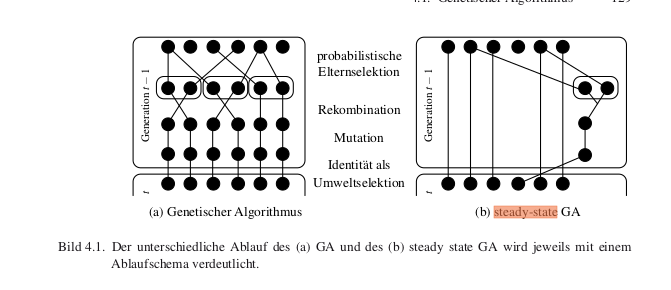
\includegraphics[scale=0.5]{img/gavssteady-state.png}
  \caption{Der unterschiedliche ablauf des a GA und des B steady state GA wird jeweils mit einem Ablaufschema verdeutlicht. Evolutionäre algorihmen s.129 }
  \label{fig:chromosome}
\end{figure}

\newpage

\subsection{Künstliche Neuronale Netze}

\begin{figure}[htb]
  \centering  
  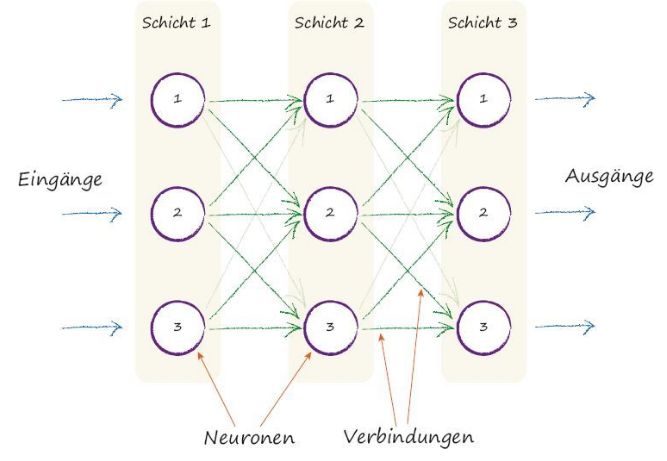
\includegraphics[scale=0.5]{img/S36_Buildyourown.png}
  \caption{Künstliches Neuronales Netz mit drei Schichten je drei Neuronen \cite{Rashid2017} }
  \label{fig:neural_network}
\end{figure}


Hier zu sehen ist ein Künstliches Neuronales Netz mit drei Schichten \ref{fig:neural_network}. Dies wurde dem natürlichen Vorbild der neuronalen Netze im Gehirn nach empfunden. Die Kreise nennt man Neuronen oder auch Perseptron, mehrere Neuronen zusammen ergeben eine Schicht oder auch Layer genannt. Die Verbindungen repräsentieren die Gewichte, über diese kann einem Netz verschiedene Zusammenhänge von Input und Output antrainiert bzw. angelernt werden. Zum Training werden viele Daten benötigt, aus welchen das Netz \glqq Lernt\grqq{}. Dafür ist es wichtig, viele aufbereitete Daten zu besitzen, denn diese Netze brauchen viele Trainingsiterationen, bis das gewünschte Ergebnis zustande kommt. Ein Neuron besteht aus Eingängen, Gewichten und einer Aktivierungfunktion sowie einem Ausgang. Die Vernetzung mehrerer Neuronenschichten lässt ein Neuronales Netz entstehen.

\newpage



\subsection{Aufbau eines Neurons}
\begin{figure}[htb]
  \centering  
  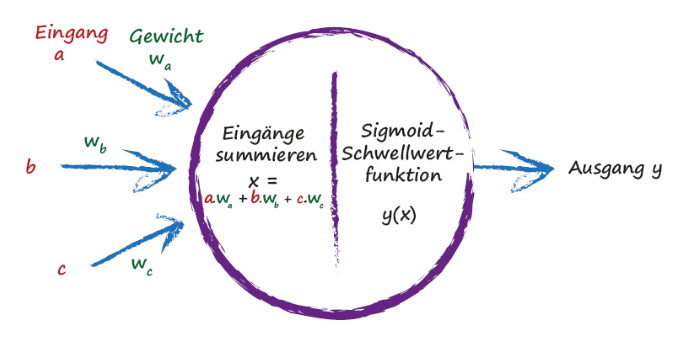
\includegraphics[scale=0.5]{img/S41_Buildyourown.png}
  \caption{Aufbau eines Neurons \cite{Rashid2017}}
  \label{fig:neuron}
  

\end{figure}
\subsubsection{Eingang aka Input}
Bei dem Input handelt es sich um einfache xxxFloatwert dieser wird mit den einzelnen Gewichten verrechnet. Ein Neuron hat meist mehrere Eingangsgrößen, welche alle zusammen mit den Gewichten aufsummiert werden. Diese Werte werden zufällig initialisiert und per Training verbessert, somit handelt es sich um einen angelernten Werte, welche durch die Backproagation(Fehlerrückführung) verbessert werden.

\subsubsection{Offset aka bias}
Auf dieses Aufsummiertes Ergebniss wird anschließend ein Bias gerechnet, dieser führt zu einem besseren Verhalten beim Trainieren. Bei diesen Werten handelt es sich um angelernte Werte, die per Backpropagation verbessert werden und die Flexibitlität der Netze erhöht.


\subsubsection{Aktivierungs Funktion}
Die Aktivierungsfunktion kann man sich als Schwellwert vorstellen, ab wann das Neuron den Input weiter gibt. Es gibt verschiedene Funktionen, um diesen Schwellwert zu definieren. Je nach Aufgabe des Neuronalen Netze werden andere Aktivierungsfunktionen verwendet. Bei Klassifizierungen werden heute meist ReLu-Layer oder ein Weakly-ReLu Layer benutzt, diese verhindern das Vanishing- bzw. Exploding- gradientproblem beim Trainieren.

\subsubsection{Ausgang aka Output}
Wenn der Schwellwert überschritten wird, wird am Output durchgeschaltet. Dieser Output kann entweder mit einer nen Schicht Neronen verbundne sein oder direkt als Ausgang gesehen werden. Über welchen man anhand von xxxVariabelenwerten/Kommawerten die 
Von Input nach Output nennt sich ein Single-Forward-Pass. Wie hier beschrieben wird, kann ein Netz verschieden viele Layer besitzen mit verschiedenen Anzahlen von Neuronen.

\subsection{Verlustfunktion aka lossfunktion}
Die Verlustfunktion stellt ein ausgesuchtes Maß der Diskrepanz zwischen den beobachteten und den vorhergesagten Daten dar. Sie bestimmt die Leistungsfähigkeit des neuronalen Netzes während des Trainings und der Ausführung. Ziel ist es, im laufenden Prozess der Modellanpassung, die Verlustfunktion zu minimieren.

\subsection{Optimierer alt Gradientenabstieg}
Um die Fehlerfunktion zu minimieren wird als Werkzeug der Gradienten Abstieg benutzt. Diese ist nur möglich da ein Künstliches Neuronales Netz aus verketteten differenzierbaren Gewichte der Neuronen(Tensoroperationen) aufgebaut ist, die es erlauben duch anwendung der Kettenregel die Gradientenfunktion zu finden, die den aktuellen Parametern des Datenstapels werte des Gradienten zuordnet. Es gibt auch hier verschiedene Ansätze von Optimierern, welche die genauen Regeln wie der Gradient der Verlustfunktion zu Aktualisierund der Parameter verwendet wird hier könnte Beispielweise den RMSProp-Optimierer, der die trägheit des Gradientenabstiegsverfahren berücksichtet.

Seite 83 - Deep Learning chollet


\iffalse
 Im Grunde werden dabei die Gewichte so angepasst, dass ein besseres Ergebnis entsteht und dadurch die Fehlerfunktion verringert wird. Wie das Wort Backpropagation schon sagt, wird von hinten nach vorne verbessert. Es gibt verschiedene Variationen von Gradientenabstiegen, welche verschiedene Vor- und Nachteile haben. Bei dem Trainieren des Netzes wurde der Momentum-Optimizer, welcher aus einem Gradientenabstieg mit Momentum aufgebaut ist.
\fi

\subsection{Hyperparameter}
Als Hyperparameter werden, in Bezug auf KNN's, meist die Anfangsbedingungen bezeichnet. Somit handelt es sich um die Learnrate (eng. Learningrate), der Abdeckunggrad(eng. Dropout), die verlustfunktion oder auch der Optimizer. In selten fällen kann man die Modelachitektur auch als Hyperparameter bezeichen. Für diese Hyperparameter gelten keine universellen Werte, sondern müssen je nach Daten und Funktion(oder KNN), speziell angepasst und verändert werden. Deshalb gibt es nur einige Regeln und grobe abschätzungen in welchem grenzen sich diese Hyperparameter befinden. 

\subsection{Zusammenfassung}





\iffalse
Genetische algorithms ist ein sehr erfolgreiches Oprimiungsverfahren welches es erlaubt auch bei schweren Suchräumen lösungen zu finden. Insbesondere wenn keine gradienten berechnet werden können. In diesem Kapitel wurden die Grundlagen der genetischen Grundlagen zusammengefasst. Sie bassieren auf einer Lösungspopulation, die sich im laufe der iterationen dem Optima annähert. Genetische Operatioren ändern die Lösungen. Cross-overoperatoren kobinieren genome zweier Lösungen. Die Mutation fügt den Lösungen Zufälligkeiten hinzu und sollte somit jenden Ort im Lösungsraum erreichen. Der Genotyp oder Das Chromosom einer Lösing wird auf einen Phänotyp, die reale Lösung, abgebildetet, bevor es mit einer Fintessfunktion ausgewertet werden kann. Diese Fittnesfunktion muss sehr sorgfällig ausgearbeitet werden, da sie einen entscheidenden einfluss auf die Suche hat. Die Lösungen mit der höchsten fittnes sind folglich die Eltern der nächsten generation. Sobald eine Generation eine bestimmte Fintess ereicht sprich genug Optimiert wurde ist die beste Lösung gefunden. Somit wurde ein Algorithmus vorgestellt welcher auf ein breites Spektrum von Probkemen anwendbar ist.

Genectic - algorhmen - essential s.19 
\fi
